\title{Big Data in Safe Driver Prediction}

\author{Jiaan Wang}
\affiliation{%
  \institution{Indiana University Bloomington}
  \streetaddress{3209 E 10 St}
  \city{Bloomington} 
  \state{IN} 
  \postcode{47408}
}
\email{jervwang@indiana.edu}

\author{Dhawal Chaturvedi}
\affiliation{%
  \institution{Indiana University Bloomington}
  \streetaddress{2679 E 7th St}
  \city{Bloomington} 
  \state{Indiana} 
  \postcode{47408}
}
\email{dhchat@iu.edu}
    
\begin{abstract}

    For years, people have been trying to reduce their automobile
    insurance bills. Insurance companies claim that price will be
    reduced for good drivers and raised for bad ones. However,
    inaccuracies in their data predictions lead to the exact
    opposite. The dataset being used is released by Porto Seguro,
    an auto and homeowner insurance company from Brazil. It
    consists of information from several hundred thousands of
    policyholders. The goal is to predict the probability an auto
    insurance policyholder files a claim the next year using
    classification algorithms. A good prediction with decent
    accuracy can correctly adjust prices for policyholders.
    
\end{abstract}

\keywords{i523, HID233, HID204, Big data, Classification, Safe Driving, Predictive Analytics, Neural Networks}

\maketitle

\section{Introduction}

Everyday, people die from car accidents and it should come as no surprise that automobile accidents are one of the most common causes of death in the United States \cite{Suizo2015decisions}. As reported by the CDC, Centers for Disease Control, approximately over 40,000 people lose their lives to fatal automobile accidents each year. It should be clear that we need to enhance road safety for drivers all over the states \cite{Mills2017safety}. However, as we are currently in the age of big data, these automobile accidents could be prevented by using modern technologies and methods such as artificial intelligence and predictive analytics. 

Big data describes large quantities of data that are impossible to analyze using traditional data analysis methods. It includes structured and unstructured data. Structured data can be SQL database stores and unstructured data can be videos, images, social media feeds, etc. In industries, data analytics is often performed on big data in order to find specific patterns or anomalies that could prove useful for business decisions and choices. The amount of data is usually irrelevant in these cases. For example, smart cars utilize big data to improve their safety features and systems. They collect data such as driving patterns and routes as they travel from point A to B. This information is then sent to the computers on-board and gets transferred to the company servers where the data undergo analysis. The result is then collected and stored to enhance smart-car systems \cite{Walker2017safety}.

Big data is also helpful in providing insights for product development. It can find the causes for issues and problems in products through data analytics, which can then be used to improve the design. For example, the driver assistance feature on a Mercedes-Benz car not only has safety features but also collects data on driving habits. If large amount of drivers speed through intersections or break hard during traffic hours, the company can obtain these information and use them properly to enhance their systems for better road safety. They could add a detector with GPS data to spot intersections or traffic jams. Furthermore, another data that are useful to collect are driving routes. Google Street View utilizes big data from driving routes to update their maps and display views of different places \cite{Walker2017safety}.

Aside from smart cars, we also need to master data collection in order to know how automobile accidents happen. For example, the technology behind the famous black box, which tracks planes and cockpit communications to determine the reason behind crashes, is getting used in cars as well. It is not expensive nor complicated to apply this technology onto the majority of vehicles out there. By recording the precise time, locations, speed and other variables, this technology can definitely help us collect valuable data and information in car accidents. The result from data analysis can also assist us in a deep understanding of causes behind automobile collisions in order to save more lives by preventing future accidents. The first country who thought to implement this technology on cars was South Korea. As a result, in the following year, a 14 percent decrease was saw in the number of car accidents along with a 20 percent decrease in the number of injuries and deaths of fatal automobile accidents \cite{Mills2017safety}.

Predictive analytics is a powerful method in big data analytics to help predict future events or outcomes based on current and historical data. It usually utilizes big data techniques such as data mining, predictive modeling and statistics. It uses a wide range of predictive models which depends on the type of event we are predicting. For example, most predictive models produce a number called a score where a higher score indicates a higher chance of that outcome happening in the future. It is a very useful tool for making business decisions and assessing potential risks in many industries such as insurance, retail, etc. Predictive analytics does not inform users about things that has happened before today. It tries to predict for a particular driver the probability that he or she may be involved in an car accident in the near future or any other chose time as accurately as possible \cite{Suizo2015decisions}.

For example, in order to find high-risk drivers, it is not enough to just have driving records, automobile incident reports or traffic tickets. We also need something called telematics. Telematics is defined as the combination of telecommunications and informatics. It collects, stores, sends and receives data and information via transmission-enabled devices. For example, the use of the car black box technology mentioned previously to collect and obtain information on driving behaviors or patterns is called vehicle telematics. With telematics data, insurance companies can determine the possibility of a driver in a future car accident along with the expenses coupled with it. They can also take actions such as putting high-risk drivers into training schools to correct their bad driving behaviors before an incident happens. 


``Using safety as an example, by analyzing a driver’s particular driving style via telematics data, a safety report can be compiled highlighting the risks inherent to the driver and help coach safer driving habits. Drivers are classified into categories of risk based off the probability that a driver will be in a collision. By making these probabilities easy to assess, a safety score can help fleets make better decisions on how to prioritize risk within their operations. The primary objectives of a safety score would be to identify risky drivers prior to a collision to provide the driver an opportunity to modify those behaviors and prevent the collision from occurring'' \cite{Suizo2015decisions}.

``Like other types of risk assessment programs, predictive analytics is not intended to be a magic bullet. It is only the beginning and requires a total commitment from the organization, fleet personnel, and driver to turn the model’s efficacy into reality. It requires strong management commitment in order to succeed. The most successful users are organizations that involve all departments in the process at an early stage including operations, safety, HR and IT. One reason previous predictive analytics projects have failed is due to the failure to achieve alignment and full enterprise adoption'' \cite{Suizo2015decisions}.

``The main component in leveraging fleet analytics is assembling and analyzing actual fleet data. In order to develop accurate and valuable predictive models, it’s important to understand the challenges you want to address first to ensure that the models are solving a real-world problem. Real data and real problems are the key'' \cite{Suizo2015decisions}.

``Start by choosing the area of greatest need (e.g., safety, maintenance, or workers compensation). Large volumes of data can result in hours of analysis with no real return in the way of fleet operational and cost optimization. One step to curb data overload is to simply ensure the data accumulated is the data actually needed. Data and analytical models should align with overall fleet goals and provide measurable and meaningful results. One good place to start leveraging analytical data is to understand your organization’s goals beyond fleet as well. Being able to meet these goals through the use of measurable analytics is the objective'' \cite{Suizo2015decisions}.

``Next, identify the key elements and the type of data that will make up your fleet’s predictive model. The necessary data is then extracted, which should be validated by the fleet. Analytics involves more than just having the data — fleets must ensure they understand what the data is telling them and why it will help them predict a future event'' \cite{Suizo2015decisions}.

``The best way to balance the accuracy and timeliness of the predictive model, such as the driver safety score described earlier, is to run the models every few weeks or the time frame that makes the most sense for your operations. Giving it at least a few weeks provides safety and operational groups enough time to take action, while still accurately reflecting the changes that indicate risk. This is balanced with trying to minimize operational burden since most have limited time, whether it’s coaching drivers or needing to get a vehicle in for repair before a major breakdown'' \cite{Suizo2015decisions}.

``To further the safety example, the program’s success could be measured by the percentage of drivers involved in collisions that were predicted accurately in the 90-day period prior to the collision. More specifically, it would examine the data of the risky driver to determine if that individual was classified at the highest risk level at least one-third of the time in the 90 days prior. This example uses an odds ratio, which is the measure of association between an exposure and an outcome. To explain further, it looks at the odds a driver will get into a collision in the next 90 days given a particular score'' \cite{Suizo2015decisions}.

``Although predictive analytics is most commonly used with fleets who were early adopters of telematics, it is something that more and more fleets are seeing the value in. With predictive analytics, fleets can proactively take action and make educated decisions that positively impact their organizations by reducing risk, whether tied to improving safety and costs or decreasing the work behind the decision-making process'' \cite{Suizo2015decisions}.

\section{Big data in auto insurance}

``For years, insurance companies have used estimates of your annual mileage to determine your car insurance rates. But with recent changes in technology, insurers now have an unprecedented ability to judge your actual driving habits. Armed with detailed data on how often you slam on the brakes and what times of day you're on the road, insurance companies are increasingly relying on precise, technological means of assessing risk — and using that information to set your monthly premiums'' \cite{Fung2016turn}.

``Traditional car insurance prices all start at the same place: risk pools. Customers are categorized by demographics such as age and sex and then the company makes guesses based on statistics about their predicted risk of future accidents. That means the rates you get are only as good as whatever information the company chooses to include in your “profile”. And that data usually has very little to do with how you actually drive. The price you pay is mostly based on the historical risk of other people who have similar profiles. Some of the risk factors make sense - like if you have previously filed several claims, you’re probably more likely to have one again in the future. Others, however, such as education or whether or not you drive an imported car, have less to do with your driving habits but still count toward your price. And the most useful measure of risk - your actual driving behavior - that’s hardly used by anyone'' \cite{Rippe2017unfair}.

``Major car insurance carriers have access to vast quantities of information and computational power, used for the purpose of determining risk, coverage, and premiums. It’s a complex affair, involving figuring out how to condense a dozen or more different factors into a single price. But you might not realize just how much Big Data goes essentially unused - representing a missed opportunity for traditional carriers. These providers use a number of different methods to compute rates for the various forms of coverage sold to drivers, but not all of these systems perform as optimally as they could. A recent study of the uses of data mining in auto insurance found that there are more accurate possible methods of identifying high-risk drivers and separating them from low-risk drivers, including one recent model incorporating 16 risk factors to provide extremely high accuracy in risk appraisal'' \cite{Rippe2017unfair}.

``The shortcomings of traditional car insurance aren’t inevitable. Today, there are easier ways for good drivers to get the premiums they deserve. Root is the first fully mobile car insurance company designed to fit your on-the-go lifestyle, insuring only good drivers in order to ensure the best rates. Our mobile-first approach fits your on-the-go lifestyle - no clunky proprietary devices are needed, only the app. Drive with Root onboard for two to three weeks, and we’ll deliver you a personalized quote based on your unique driving data. You can easily select the coverage you want to buy and pay immediately via your phone. It’s that simple'' \cite{Rippe2017unfair}.

``Usage-Based Insurance (UBI), a somewhat recent innovation by auto insurers, closely aligns driving behaviors with premium rates for auto insurance. Mileage and driving behavior can be captured by applications on your smartphones as well as OBD devices or embedded in-car technology provided directly by the auto manufacturer. With the first UBI programs, insurance companies provided insurance discounts to reward good driving behavior. Now those discounts are combined with other rewards and benefits like roadside assistance and vehicle theft recovery. By capturing big data around driving behavior, insurance companies will be able to quickly determine fault when accidents do occur. Insurance companies will be able to do this by understanding precise movements of each car, combining behavioral data, such as hard braking and accelerating, with real-time contextual data, including road conditions and the weather, and even video from on-board cameras'' \cite{Shafer2016industry}.

``Increasingly, Big Data – make that Big Brother? – is in the front seat of your car, and is affecting how much you pay for auto insurance. In theory, “usage-based” or “pay-as-you-drive” insurance sounds perfectly reasonable and fair. Instead of profiling drivers based just on the traditional factors—age, location of residence, history of accidents and traffic violations, and so on—a small device is installed into the car that monitors how drivers actually drive. These programs, including Allstate’s “Drivewise” and Progressive’s “Snapshot,” have been available for several years in select locations on a strictly voluntary basis. Drivers have been welcoming these devices into their cars because, at least for now, they’re being presented on a “discount only” basis. That is, drivers whose habits are deemed to be sufficiently safe—easy on the brakes and gas pedal, limited long-haul trips or driving during “risky” hours—can see their premiums drop by 5 percent, 10 percent, sometimes upwards of 30 percent. On the downside, consumer advocates worry that these devices cause drivers to give up their privacy, and that no one really knows what the long-term repercussions could be by welcoming insurance companies inside cars. Just about every article written on the topic includes the phrase Big Brother. Now, reports the Wall Street Journal, these programs are expanding in a big way. State Farm, the country’s largest auto insurer, has plans to promote its “Drive Safe and Save” program in nearly every state by the end of 2013. The main selling point is that by accepting these devices in their vehicles, customers can prove that they’re safe drivers who deserve cheaper insurance rates'' \cite{Tuttle2013habits}.

``One of the first usage-based insurance (UBI) programs to hit the market was Progressive’s partnership with General Motors roughly a decade ago. The program implemented a mileage-based discount to users by using GPS technology. Many UBI programs still use this technology, but there have been many advancements. Insurers can now know how, where, and when policyholders drive. UBI variations include “pay as you drive” (PAYD), “pay how you drive” (PHYD), and other distance- and telematics-based insurance options. The term “telematics” refers to the merging of telecommunications and information science for accurate data assessment. The benefits of telematics-based UBI programs include the ability to increase accident response time and track lost or stolen vehicles. Additionally, a popular method of analyzing UBI is through plug-in devices. These devices, which connect via the OBD-II port of a car, don’t necessarily track location, but they do report more accurate and detailed information about vehicle usage. While telematics and GPS are the most common ways to track driving behaviors, future innovations will likely include using a car or phone’s GPS and accelerometer to monitor abrupt alterations in speed and other unsafe behavior. In December 2015, Liberty Mutual tested volunteer drivers with this technology in order to expand their RightTrack program, and State Farm is testing their own voluntary phone tracking platform. According to SMA Research, it is expected that nearly 70 percent of all auto insurance carriers will use telematics-based UBI by 2020. UBI methods are on the rise and will continue to grow in accuracy and accessibility'' \cite{Firm2016insurance}.

``On a different scale, the connected car is changing the way companies view automotive insurance. Vehicles today send thousands of data points to servers every second, detailing everything from their location to braking and their speed. In the future, vehicle-to-infrastructure solutions will communicate high-resolution road conditions—down to the pothole and puddle level—on a real-time basis. Insurance companies can use this data to make real-time decisions that manage risk, perhaps even using telematics and automated-driving technology to advise drivers on the least dangerous route to take. The use of big data in insurance is already transforming the industry. For example, Ford has partnered with IVOX, developer of the DriverScore app. This uses privacy-enhanced technology to tell insurance companies how drivers are performing in order to potentially lower their premiums. Similarly, connected homes are getting better at communicating their environmental conditions'' \cite{Bradbury2017game}. 

``One of the most important uses is for setting policy premiums. In insurance, efficiency is an important keyword. Insurers must set the price of premiums at a level which ensures them a profit by covering their risk, but also fits with the budget of the customer – otherwise they will go elsewhere. A great example of this formula in action is motor insurance. While drivers (particularly younger ones) often complain about the high prices, this is a market where there is a huge amount of competition and shopping around on price comparison services is common among customers. As a result an insurance business is made or broken on its ability to accurately assess the risk posed by a particular driver and offer them a competitive, but profit-making premium'' \cite{Marr2015forever}.

``Many insurers now offer telemetry-based packages, where actual driving information is fed back to their system to a personalized, highly accurate profile of an individual customer’s behavior can be built up. Using predictive modelling as mentioned above, the insurer can work out an accurate assessment of that driver’s likelihood to be involved in an accident, or have their car stolen, by comparing their behavioural data with that of thousands of other drivers in their database. This data is sometimes captured and transmitted from a specially installed box fitted to the car or, increasingly, from an app on a driver’s smart-phone. US insurers Progressive offer a great example of a business which has committed to working with data to enhance its services. It has created what is calls its Business Innovation Garage where technologists known as “mechanics” produce and road-test innovations. One project involves rendering 3D images of damaged vehicles using computer graphics. Images are scanned in from cameras to create 3D models allowing structured data to be recorded on the condition and damage to a vehicle'' \cite{Marr2015forever}.

\section{Current Applications}

``Predictive analytics are being employed in interesting new ways to improve safety. Telematics solutions have long monitored events like hard braking and speeding to flag unsafe driver behaviors.  But today, this driver event data is being enriched with other data streams to actually predict the likelihood of a specific driver having an accident. A company called SmartDrive Systems goes even further in their efforts to predict accidents.  They are enriching the telematics data with video feeds from road facing and interior facing cameras.  The company is combining asset sensor with driver sensor data to do better driver safety analytics and ultimately make better predictions'' \cite{Banker2016accident}.

``SmartDrive Systems is a predictive analytics supplier whose solution is based on a private cloud architecture.  In other words, all of their customers’ data is captured by the company; they have telematics and video on four billion miles driven, of which they scored almost 200 million events.   SmartDrive’s customer agreements allow them to analyze all the customer data so they can continue to improve their algorithms.  “We are constantly tuning and improving our algorithms,” Mr. Mitgang said. The combination of telematics and video has allowed their scientists to better interpret the telematics data. By reading the telematics data, and seeing what happened, they were able to determine, for example, that turning more than 165 degrees within a certain turning radius and time window was a risky U-turn on a roadway. SmartDrive also detected additional patterns to avoid false trigger activation in large open areas such as parking lots and truck stops'' \cite{Banker2016accident}.

``Indiana State Police decided to take a different approach, and are making their predictive crash analytics program available to the public, as well as troopers. A color-coded Daily Crash Prediction map, which went online in November, pulls together data that includes crash reports from every police agency in the state dating to 2004, daily traffic volume, historical weather information and the dates of major holidays, said First Sgt. Rob Simpson. The online map pinpoints where a crash is likely, ranging from a very low to a high probability. It also highlights prior crash sites and displays information about the date and cause, whether EMS was called, if there was a fatality, and if drugs or alcohol were involved. As of late January, the site had nearly 4,800 page visits'' \cite{Bergal2017sites}.

``Liberty Mutual, the country's third-largest property-and-casualty insurer, took the latest step in that direction Monday when it announced a partnership with Subaru. Beginning later this year, Subaru drivers who have paid for the automaker's Starlink infotainment system will be able to download an app to their cars that notifies them when they are accelerating too aggressively or braking too hard. The app is part of Liberty Mutual's RightTrack program, which gives drivers a 5 percent discount on their rates for enrolling and additional discounts up to 30 percent for heeding the app's guidance on driving safely'' \cite{Fung2016turn}. 

\section{Data Analysis}
The data we are gonna use for our analysis is of Porto Seguro. It is one of Brazil's largest auto and homeowner insurance companies. Inaccuracies in car insurance company's claim predictions raise the cost of insurance for good drivers and reduce the price for bad ones. The task is to build a model that predicts the probability that a driver will initiate an auto insurance claim in the next year or not. An accurate prediction will allow them to further tailor their prices, and hopefully make auto insurance coverage more accessible to more drivers. 
\\
\subsection{Approach}
We will be mainly discussing about the Exploratory data Analysis we have  performed on the data until now. We will be using the help of both R and python environment and supporting packages to perform the necessary statistical analysis. Along with this, we will discuss  about  the  Machine  or  Deep  Learning  algorithms  / models that we will be using to achieve the near solution for the problem.

\subsection{Feature Information}
\ Dimensions of the data [Rows x Features] : [ 595212, 59 ]
\\ \newline The dataset constitutes different varieties of features.
\\ \newline \textbf{Binomial Features} [Count : 17] :  ps\_ind\_06\_bin,  ps\_ind\_07\_bin, ps\_ind\_08\_bin, ps\_ind\_09\_bin, ps\_ind\_10\_bin, ps\_ind\_11\_bin, ps\_ind\_12\_bin, ps\_ind\_13\_bin, ps\_ind\_16\_bin, ps\_ind\_17\_bin, ps\_ind\_18\_bin, ps\_calc\_15\_bin, ps\_calc\_16\_bin, ps\_calc\_17\_bin, ps\_calc\_18\_bin, ps\_calc\_19\_bin, ps\_calc\_20\_bin.
\
\\ \newline \textbf{Categorical Features} [Count : 14] : ps\_ind\_02\_cat,  ps\_ind\_04\_ cat, ps\_ind\_05\_cat, ps\_ind\_01\_cat, ps\_ind\_02\_cat,  ps\_ind\_03\_cat, ps\_ind\_04\_cat, ps\_ind\_05\_cat, ps\_ind\_07\_cat,  ps\_ind\_06\_cat, ps\_ind\_08\_cat, ps\_ind\_09\_cat, ps\_ind\_10\_cat,  ps\_ind\_11\_cat.
\
\\ \newline \textbf{Integer Features} [Count : 16] : ps\_ind\_01, ps\_ind\_03, ps\_ind\_14, ps\_ind\_15, ps\_ind\_11, ps\_calc\_04, ps\_calc\_05, ps\_calc\_06, ps\_calc\_07, ps\_calc\_08, ps\_calc\_09, ps\_calc\_10, ps\_calc\_11, ps\_calc\_12, ps\_calc\_13, ps\_calc\_14.
\
\\ \newline \textbf{Floating Features} [Count :10] : ps\_reg\_01, ps\_reg\_02, ps\_reg\_03, ps\_calc\_01, ps\_calc\_02, ps\_calc\_03, ps\_car\_12, ps\_car\_13, ps\_car\_14, ps\_car\_15.
\\ \newline  The remaining two features constitutes \textbf{id} and the \textbf{output (or) target}. 
\\ \newline All the features has been clearly represented using post script, \textbf{\_cat} for categorical data, \textbf{\_bin} for binomial data.
\\ \newline The \textbf{missing values} in the features are represented by -1.

\subsection{Data Preprocessing}
As shown in \ref{f:missing}, missing values are found in 14 of the 58 columns. There are 6 features with more than 5000 missing row values. Owing to the shear size of the unavailable data, we have not performed any missing value treatment and removed these features from consideration. Of the remaining data, across rows, data is unavailable in atmost 500 ($<$1\%) rows and these are promptly removed.

\begin{figure}[!ht]
  \centering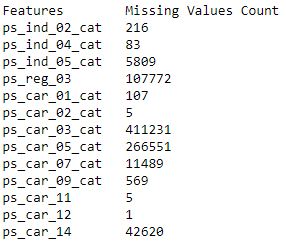
\includegraphics[width=\columnwidth]{images/missingdata.PNG}
  \caption{Missing Data}\label{f:missing}
\end{figure}

\subsection{Distribution of the target variable}
As shown in \ref{f:numerical}, target variable claims is a binary variable with a skewed distribution of classes. 96\% of the customers didn't make any claims. We wish to consider this distribution in measuring classification accuracy. Area under the ROC curve, recall and precision would be relevant metrics in this case.
 
\begin{figure}[!ht]
 \centering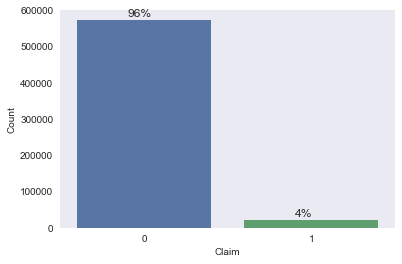
\includegraphics[width=\columnwidth]{images/target.png}
 \caption{Target Variable Distribution}\label{f:numerical}
\end{figure}

\subsection{Numerical Predictors (vs) Target Variable}
 Average value of most of the numerical predictors is higher when the claims are filed. This is a unique phenomenon and we intend to use this contrast in predicting the target variable.
  
\subsection{Artificial Neural Networks}
Artificial neural networks (ANNs)  are computing models which are based on biological neural networks that constitute human brains. The idea of ANNs is based on the belief that working of human brain can be imitated for computers by using silicon and wires as living neurons. Such systems learn by progressively improving their performance to do tasks by considering examples, generally without task-specific programming. The human brain can be considered as a complex network of nerve cells called neurons(about 86 billion). They are inter-connected to other millions of cells by Axons. These neurons then react to stimulation from external environment or inputs from other organs. A neuron can then send the message to other neuron to handle the issue or does not send it forward. 
\\
ANNs also try to imitate biological neurons of human brain. The neurons are connected by links and they interact with each other. The nodes can take input data and perform simple operations on the data. The result of these operations is passed to other neurons. The output at each node is called its activation. Each node is assigned with weight. ANNs are capable of learning, which takes place by altering weight values. If the network generates the desired output, there is no need to adjust the weights. However, if the network generates an undesired output or an error, then the system alters the weights in order to improve subsequent results.

\subsection{Types of ANNs}
\subsubsection{Feedback ANN}
In these type of ANN, the output goes back into the network to achieve the best-evolved results internally. The feedback network feeds information back into itself and is well suited to solve optimization problems. Feedback ANNs are used by the Internal system error corrections. 
\subsubsection{Feed Forward ANN}
A feed-forward network is a simple neural network consisting of an input layer, an output layer and one or more layers of neurons.Through evaluation of its output by reviewing its input, the power of the network can be noticed base on group behavior of the connected neurons and the output is decided. The main advantage of this network is that it learns to evaluate and recognize input patterns.
\subsubsection{Radial Basis Function Neural Network}
The RBF neural network is the first choice when interpolating in a multidimensional space. The RBF neural network is a highly intuitive neural network. Each neuron in the RBF neural network stores an example from the training set as a “prototype”. Linearity involved in the functioning of this neural network offers RBF the advantage of not suffering from local minima.
\subsubsection{Kohonen Self-Organising Neural Network}
Invented by Teuvo Kohonen, the self-organizing neural network is ideal for the visualization of low-dimensional views of high-dimensional data. The self-organizing neural network is different from other neural networks and applies competitive learning to a set of input data, as opposed to error-correction learning applied by other neural networks. The Kohonen self-organizing neural network is known for performing functions on unlabeled data to describe hidden structures in it.
\subsubsection{Recurrent Neural Network}
The recurrent neural network, unlike the feed forward neural network, is a neural network that allows for a bi-directional flow of data. The network between the connected units forms a directed cycle. Such a network allows for dynamic temporal behavior to be exhibited. The recurrent neural network is capable of using its internal memory to process arbitrary sequence of inputs. This neural network is a popular choice for tasks such as handwriting and speech recognition.
\subsubsection{Classification-Prediction ANN}
It is the subset of feed-forward ANN and the classification-prediction ANN is applied to data-mining scenarios. The network is trained to identify particular patterns and classify them into specific groups and then further classify them into “novel patterns” which are new to the network.
\subsubsection{Physical Neural Network}
This neural network aims to emphasize the reliance on physical hardware as opposed to software alone when simulating a neural network. An electrically adjustable resistance material is used for emulating the function of a neural synapse. While the physical hardware emulates the neurons, the software emulates the neural network.

\subsection{Data Analysis Using Neural Networks}
Rather than beginning our inquiry into the dataset with more traditional methods like regression we straight away tried to learn Artificial Neural Networks. Logistic regression itself, can be thought of as a special case of a neural network with a single neuron (~perceptron). 
\\
After studying and learning the theory behind ANNs we proceeded to learn how to implement them -- by ourselves at first, and later using TensorFlow. So far we have tried quite a bit of different models and learnt some lessons about the data.
\\
\begin{itemize}
\item \textbf{Data Cleaning :} As pointed out by the EDA above, there were a few columns which had a lot of missing data. For columns which had $>1000$ values missing (~6 columns), we disregarded them altogether. For the remaining data points, we disregarded the rows which had any one particular value missing. We started with a simple data cleaning strategy so as to not complicate it too much at the initial stages, but we will probably want to look at it again as we go along.

\item The first thing that we tried is using a simple \textbf{perceptron}. The input layer had 51 nodes (after removing the id, target and 6 other columns in data cleaning) and the output layer had a single perceptron with a sigmoid activation function. The best score that we got when we uploaded our code to kaggle was $0.03$ whereas the leaderboard is hovering around $0.290$ so this is not too impressive.

\item However, now we added more hidden layers and nodes to see if we get a better job of fitting the data. To start off, we only consider the continuous variables so that we don't have to worry about handling binary/categorical data. We have $24$ nodes in the input layer. The final layer has one node  since it is a classification problem. We kept all activations to be logistic and experimented a bit with the number of hidden layers and nodes to get a best score of \textbf{0.211} with this simple approach.

\item \textbf{Issued Encountered}  Looking at the results from the neural network there is one major issue. Whenever we add too many hidden layers ($>3$) the outputs for the test data are all $\approx 0$ and the score drops. After some trial and error, we have diagnosed the issue to be the biased nature of the training data (~$96\%$ of the training data are $0's$). So the ANN sees too many zeros and consequently predicts mostly zeros. We aim to explore different sampling methods to train the neural network to improve the results further (along with cross validation which we haven't implemented).
\end{itemize}


\section{Other Techniques that can be used}
Among the machine Learning algorithms that are used in practice, gradient tree boosting is one technique that shines in many applications.Tree Boosting has been shown to give many state of the art results for many standard classification problem.
\\
The most important factor for the success of XGBoost is its ability to scale in all the scenarios. The XGBoost algorithm run ten times faster than the existing popular solutions on a single solution and scales to billions of example in distributed or memory-limited settings.
\\
The Porto Seguro dataset is clearly an classification problem, The data will be having only two outputs either the car insurance holder is going to claim or not.
\\
While domain dependent analysis and feature engineering plays an important role in defining or modeling the solutions, the fact that XG Boost is the consensus choice for learners shows the impact and importance of our system in tree boosting.One problem with the Porto Seguro dataset we dont have have much information about the Features and all the feature must have to under go through strict statistical treatment to build an optimal solution.

\section{Conclusion}


\begin{acks}

  The authors would like to thank Dr. Gregor von Laszewski for his
  support and suggestions to write this paper.

\end{acks}

\bibliographystyle{ACM-Reference-Format}
\bibliography{report} 
